\documentclass[border=0pt]{standalone}
\usepackage[T1]{fontenc}
\usepackage{mathptmx}
\usepackage{amsmath}
\usepackage{tikz}
\usetikzlibrary{backgrounds,shapes.geometric}
% Multilayer MCTDHF ansatz drawn as a layered graph: nodes are functions,
% coloured edges carry the variational coefficients (b, B, A), thin black
% edges are fixed products (antisymmetrized within a species, tensor across).
% Example: K = 2 species, N_sigma = 2 particles, M_sigma = 3 orbitals
% (3 determinants), n_s = 2 SBS per species.
\definecolor{cb}{RGB}{0,114,178}    % b   (orbitals)
\definecolor{cB}{RGB}{0,158,115}    % B   (SBS)
\definecolor{cA}{RGB}{213,94,0}     % A   (top tensor)
\begin{document}
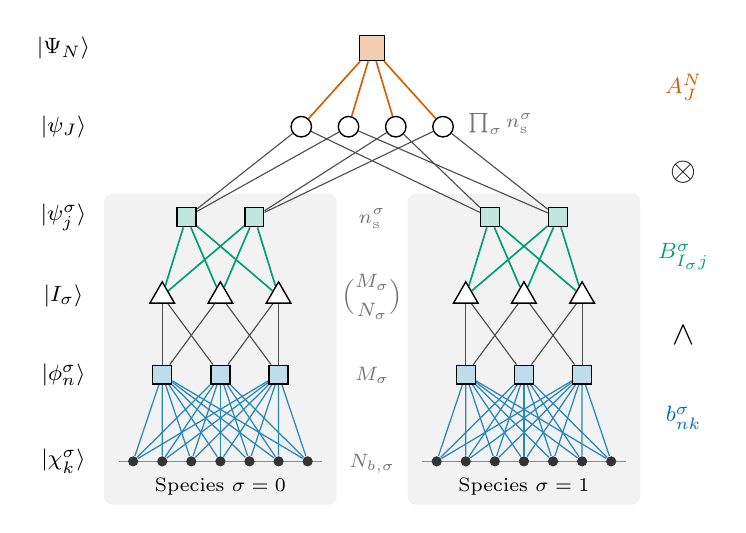
\begin{tikzpicture}[
  font=\footnotesize,
  lin/.style={rectangle, draw, line width=0.5pt, minimum size=2.4mm, inner sep=0pt},
  det/.style={regular polygon, regular polygon sides=3, draw, line width=0.5pt, fill=white, minimum size=3.6mm, inner sep=0pt},
  prd/.style={circle, draw, line width=0.5pt, fill=white, minimum size=2.6mm, inner sep=0pt},
  pt/.style={circle, fill=black!80, minimum size=1.3mm, inner sep=0pt},
  coef/.style={line width=0.6pt},
  prod/.style={line width=0.4pt, black!70},
  lab/.style={anchor=center},
  rlab/.style={anchor=center},
  spec/.style={rounded corners=3pt, fill=black!5, draw=none}]
% layer heights
\def\yc{0}\def\yp{1.1}\def\yi{2.1}\def\ys{3.1}\def\yJ{4.25}\def\yP{5.25}
% species centres and the centre of the register
% \hw is the half-width of a species box; the figure is sized to the
% 246pt column width of the paper through \hw
\def\hw{1.4775}\def\gap{0.9}
\pgfmathsetmacro\sc{\hw/1.2}
\pgfmathsetmacro\cz{\hw}
\pgfmathsetmacro\co{3*\hw+\gap}
\pgfmathsetmacro\cm{2*\hw+\gap/2}

% ---------- nodes. Squares are linear combinations of the layer below
% (filled in the colour of their coefficients), triangles are determinants
% (antisymmetrized products) and circles are tensor products.
\foreach \c/\s in {\cz/0,\co/1}{
  % primitive basis chi_k: DVR grid points on the species' grid
  \draw[black!45, line width=0.4pt] (\c-1.05*\sc,\yc) -- (\c+1.05*\sc,\yc);
  \foreach \k in {1,...,7}
    \node[pt] (x\s\k) at ({\c+0.3*\sc*(\k-4)},\yc) {};
  % orbitals phi_n
  \foreach \p/\dx in {1/-0.6,2/0,3/0.6}
    \node[lin, fill=cb!25] (p\s\p) at (\c+\dx*\sc,\yp) {};
  % determinants I_sigma = |phi_1 phi_2|, |phi_1 phi_3|, |phi_2 phi_3|
  \foreach \i/\dx in {1/-0.6,2/0,3/0.6}
    \node[det] (i\s\i) at (\c+\dx*\sc,\yi) {};
  % SBS psi^sigma_j
  \foreach \j/\dx in {1/-0.35,2/0.35}
    \node[lin, fill=cB!25] (s\s\j) at (\c+\dx*\sc,\ys) {};
}
% product SBS psi_J, J = (j_0, j_1)
\foreach \a/\b/\dx in {1/1/-0.9,1/2/-0.3,2/1/0.3,2/2/0.9}
  \node[prd] (J\a\b) at (\cm+\dx,\yJ) {};
% state
\node[lin, minimum size=3.2mm, fill=cA!30] (Psi) at (\cm,\yP) {};

% ---------- species backgrounds and edges, behind the nodes
\begin{pgfonlayer}{background}
\foreach \c/\s in {\cz/0,\co/1}{
  \fill[spec] (\c-\hw,\yc-0.55) rectangle (\c+\hw,\ys+0.3);
  \node[font=\scriptsize] at (\c,\yc-0.32) {Species $\sigma=\s$};
}
\foreach \s in {0,1}{
  % b: chi_k -> phi_n, all-to-all
  \foreach \k in {1,...,7}
    \foreach \p in {1,2,3}
      \draw[line width=0.45pt, cb!85] (x\s\k) -- (p\s\p);
  % antisymmetrized products phi -> I
  \foreach \i/\pa/\pb in {1/1/2,2/1/3,3/2/3}{
    \draw[prod] (p\s\pa) -- (i\s\i);
    \draw[prod] (p\s\pb) -- (i\s\i);
  }
  % B: I_sigma -> psi^sigma_j, all-to-all
  \foreach \i in {1,2,3}
    \foreach \j in {1,2}
      \draw[coef, cB] (i\s\i) -- (s\s\j);
}
% tensor products psi^0_{j0} (x) psi^1_{j1} -> psi_J
\foreach \a in {1,2}
  \foreach \b in {1,2}{
    \draw[prod] (s0\a) -- (J\a\b);
    \draw[prod] (s1\b) -- (J\a\b);
  }
% A: psi_J -> Psi_N
\foreach \a in {1,2}
  \foreach \b in {1,2}
    \draw[coef, cA] (J\a\b) -- (Psi);
\end{pgfonlayer}

% ---------- layer labels (left): the functions
\def\xl{-0.515}
\node[lab] at (\xl,\yc) {$|\chi^{\sigma}_{k}\rangle$};
\node[lab] at (\xl,\yp) {$|\phi^{\sigma}_{n}\rangle$};
\node[lab] at (\xl,\yi) {$|I_{\sigma}\rangle$};
\node[lab] at (\xl,\ys) {$|\psi^{\sigma}_{j}\rangle$};
\node[lab] at (\xl,\yJ) {$|\psi_{J}\rangle$};
\node[lab] at (\xl,\yP) {$|\Psi_{N}\rangle$};

% ---------- layer sizes, in the gap between the species
\tikzset{num/.style={anchor=mid, font=\scriptsize, black!55, inner sep=1pt}}
\node[num] at (\cm,\yc) {$N_{b,\sigma}$};
\node[num] at (\cm,\yp) {$M_{\sigma}$};
\node[num] at (\cm,\yi) {$\dbinom{M_\sigma}{N_\sigma}$};
\node[num] at (\cm,\ys) {$n^{\sigma}_{\mathrm s}$};
\node[num, anchor=mid west] at (\cm+1.18,\yJ+0.06) {$\prod_\sigma n^{\sigma}_{\mathrm s}$};

% ---------- edge labels (right): the coefficients / products
\pgfmathsetmacro\xr{4*\hw+\gap+0.55}
\node[rlab, cb] at (\xr,{(\yc+\yp)/2}) {$b^{\sigma}_{nk}$};
\node[rlab]     at (\xr,{(\yp+\yi)/2}) {\large$\wedge$};
\node[rlab, cB] at (\xr,{(\yi+\ys)/2}) {$B^{\sigma}_{I_\sigma j}$};
\node[rlab]     at (\xr,{(\ys+\yJ)/2}) {\large$\otimes$};
\node[rlab, cA] at (\xr,{(\yJ+\yP)/2}) {$A^{N}_{J}$};
\end{tikzpicture}
\end{document}
